% [原文 p.155]
\[
  \overline{x}\in G^{2q}K(X)\otimes\Z/p
\]
这一元素。这里，由于 $X$ 无挠，回想存在分次环的同构
\[
  H^*(X;\Z)\cong GK^*(X)
\]
（见 [8, §2]），便得到
\[
  H^{2q}(X;\Z/p)\cong G^{2q}K(X)\otimes\Z/p.
\]
通过这个同构，算子 $x\mapsto\overline{x_i}$ 必须对应某个上同调算子。下一节将证明，它恰好就是 Steenrod 算子 $P^i_p$。

% [Tutor Note: $H^*(X;\Z)\Rightarrow K^*(X)$ 中的双箭头指 Atiyah–Hirzebruch 谱序列；文中“由 $a$ 代表”是说 $a$ 是 $E_2$ 页上对应 $x$ 的类，而不是 $x$ 的某个具体代表元，故这类断言只能逐次读取。]

\section{与上同调算子的关系}
\takeaway{本节把张量幂算子接入上同调：命题 B.6.4 用谱序列说明 $\alpha(x^{\otimes k})$ 与 $\nu(a)$ 对应，定理 B.6.5 则证明 $\psi^p(x)$ 的展开系数 $\overline{x_i}$ 恰为 Steenrod 算子 $P^i_p(\overline{x})$。}

在命题 B.4.2 的证明中，我们验证了包含映射
\[
  j\colon(X^k,X^k_{2kq-1})\to(X,X_{2q-1})^k
\]
存在。因此可以考察由
\[
  K(X,X_{2q-1})\to K(X^k_{S_k},(X^k_{S_k})_{2kq-1})
\]
中 $x\mapsto\alpha j^*x^{\otimes k}$ 给出的映射。把这一映射与对角映射 $X_{S_k}\to X^k_{S_k}$ 的胞腔近似复合，便得到映射
\[
  \eta\colon K(X,X_{2q-1})\to K(X_{S_k},(X_{S_k})_{2kq-1}).
\]
由定义，它与从 $K(X)$ 到 $K(X_{S_k})$ 的算子
\[
  x\mapsto d^*\alpha x^{\otimes k}=\alpha x^{\otimes k}
\]
是相容的。也就是说，图式

% [原文 p.156]
\begin{equation}
  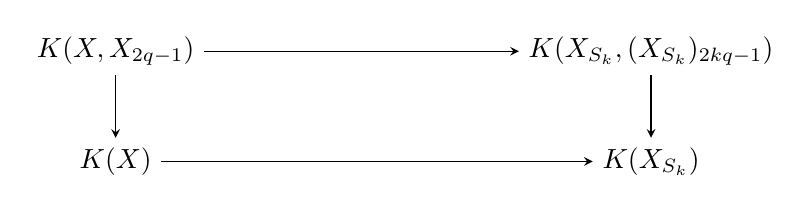
\begin{tikzpicture}[>=stealth, baseline=(current bounding box.center)]
    \node (A1) at (0,1.4) {$K(X,X_{2q-1})$};
    \node (B1) at (6.8,1.4) {$K(X_{S_k},(X_{S_k})_{2kq-1})$};
    \node (A2) at (0,0) {$K(X)$};
    \node (B2) at (6.8,0) {$K(X_{S_k})$};
    \draw[->] (A1) -- (B1);
    \draw[->] (A1) -- (A2);
    \draw[->] (B1) -- (B2);
    \draw[->] (A2) -- (B2);
  \end{tikzpicture}
  \tag{B.6.1}
\end{equation}
可交换。另一方面，把 $X$ 限制到 $X_{2q}$、把 $X_{S_k}$ 限制到 $(X_{S_k})_{2kq}$，又得到另一个交换图式
\begin{equation}
  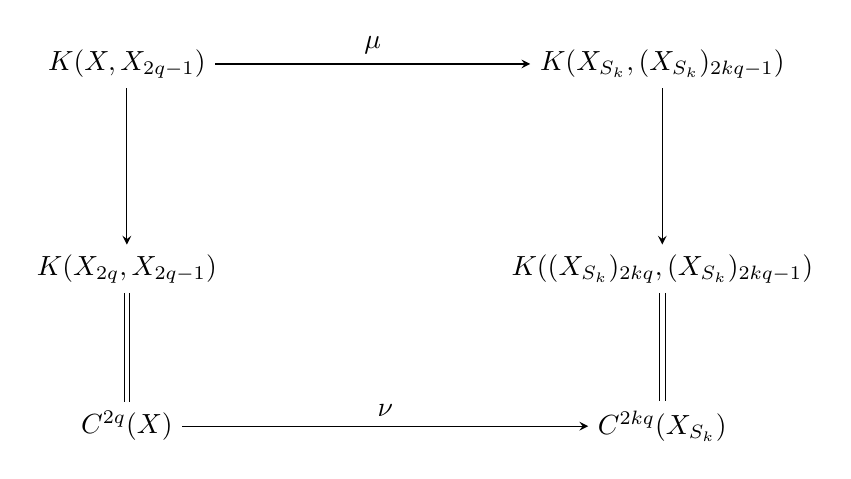
\begin{tikzpicture}[>=stealth, baseline=(current bounding box.center)]
    \node (A1) at (0,2.6) {$K(X,X_{2q-1})$};
    \node (B1) at (6.8,2.6) {$K(X_{S_k},(X_{S_k})_{2kq-1})$};
    \node (A2) at (0,0) {$K(X_{2q},X_{2q-1})$};
    \node (B2) at (6.8,0) {$K((X_{S_k})_{2kq},(X_{S_k})_{2kq-1})$};
    \node (A3) at (0,-2.0) {$C^{2q}(X)$};
    \node (B3) at (6.8,-2.0) {$C^{2kq}(X_{S_k})$};
    \draw[->] (A1) -- node[above] {$\mu$} (B1);
    \draw[->] (A1) -- (A2);
    \draw[->] (B1) -- (B2);
    \draw[double, double distance=1.6pt] (A2) -- (A3);
    \draw[double, double distance=1.6pt] (B2) -- (B3);
    \draw[->] (A3) -- node[above] {$\nu$} (B3);
  \end{tikzpicture}
  \tag{B.6.2}
\end{equation}
其中 $\nu$ 是由
\begin{equation}
  \nu(c)=d^*[(c\otimes c\otimes\cdots\otimes c)\otimes_\Gamma1] \tag{B.6.3}
\end{equation}
给出的上链映射。这里，我们把
\[
  C^*(X^k_{S_k})=(C^*(X)\otimes_\Z\cdots\otimes_\Z C^*(X))\otimes_\Gamma C^*(A)
\]
等同起来，其中 $A\to B_{S_k}$ 是万有 $S_k$ 丛，$\Gamma$ 是 $S_k$ 的整系数群环。同样地，把
\[
  C^*(X_{S_k})=C^*(X)\otimes_\Gamma C^*(A)
\]
等同起来。图式 (B.6.2) 的可交换性当然依赖于同构
\[
  K(X_{2q},X_{2q-1})\cong C^{2q}(X)
\]
与（外）积相容这一事实。

% [Tutor Note: (B.6.3) 中 $(c\otimes\cdots\otimes c)$ 是 $k$ 个 $c$ 的张量积，$\otimes_\Gamma$ 再用群环 $\Gamma$ 与 $1$ 作用，等于把 $S_k$ 的对称化一次并入；这也是为何 $\nu$ 只在 $X_{S_k}$ 一侧出现。]

(B.6.3) 定义的映射 $\nu$ 诱导上同调映射（也用 $\nu$ 表示）
\[
  \nu\colon H^{2q}(X;\Z)\to H^{2kq}(X_{S_k};\Z).
\]
于是，由图式 (B.6.1) 与 (B.6.2) 便证明了下面的命题。

\begin{proposition*}{B.6.4}
  设 $x\in K_{2q}(X)$ 在谱序列 $H^*(X;\Z)\Rightarrow K^*(X)$ 中由 $a\in H^{2q}(X;\Z)$ 代表。此时 $\alpha(x^{\otimes k})\in K_{2kq}(X_{S_k})$ 在谱序列
  \[
    H^*(X_{S_k};\Z)\Rightarrow K^*(X_{S_k})
  \]
  中由 $\nu(a)\in H^{2kq}(X_{S_k};\Z)$ 代表，其中 $\nu$ 由式 (B.6.3) 诱导。
\end{proposition*}

% [原文 p.157]
\begin{remark}{}
  (1) 把 $X$ 的谱序列写成 $X_{S_k}$ 的谱序列的张量幂算子，看来是可以定义的。命题 B.6.4 只处理两个端点的要素 $E_2$ 与 $E_\infty$（而且只对偶数维处理）。

  (2) 映射 $\nu$ 是一切 Steenrod 算子的源头，而 $x\mapsto x^{\otimes k}$ 是 B.2 节引入的 $K$ 理论一切算子的源头。因此命题 B.6.4 原则上包含了这两个理论的算子之间的全部关系。我们就在最单纯的情形下把这一关系讲清楚。
\end{remark}

\begin{theorem*}{B.6.5}
  假定 $X$ 无挠，从而可把 $H^*(X;\Z/p)$ 与 $GK^*(X)\otimes\Z/p$ 等同。用 $\overline{x}$ 表示 $H^{2q}(X;\Z/p)$ 中对应于 $x\in K_{2q}(X)$ 的元素。设命题 B.5.6 给出的 $\psi^p(x)$ 的分解为
  \[
    \psi^p(x)=\sum_{i=0}^{q}p^{q-i}x_i.
  \]
  此时
  \[
    \overline{x_i}=P^i_p(\overline{x})
  \]
  成立，其中
  \[
    P^i_p\colon H^{2q}(X;\Z/p)\to H^{2q+2i(p-1)}(X;\Z/p)
  \]
  是 Steenrod 算子（对 $p=2$，约定 $P^i_2=Sq^{2i}$）。
\end{theorem*}

% [Tutor Note: $p=2$ 时约定 $P^i_2=Sq^{2i}$，只取偶数次 Steenrod 平方；这与奇素数时 $P^i_p$ 的次数 $2i(p-1)$ 相合，若误写成 $Sq^i$ 则次数全错。]

\begin{proof}
  由命题 B.6.4，可知映射
  \[
    P\colon K(X)\to K(X)\otimes R(\Z/p)
  \]
  通过模 $p$ 的 $\nu$ 诱导出
  \begin{equation}
    \overline{P}\colon H^*(X;\Z/p)\to H^*(X;\Z/p)\otimes H^*(\Z/p;\Z/p). \tag{1}
  \end{equation}
  这里，由 (B.2.6) 与引理 B.5.5（取 $x_q=x^p$）可知
  \begin{equation}
    P(x)=x_q\otimes1-\sum_{i=0}^{q-1}x_i\otimes p^{q-i-1}(N-p). \tag{2}
  \end{equation}
  由 Steenrod 算子的定义 [10, p.112]，
  \[
    \overline{P}(\overline{x})=\sum_{i=0}^{q}(-1)^{q-i}P^i(\overline{x})\otimes\eta^{(q-i)(p-1)}
  \]
  成立，其中 $\eta$ 是 $H^2(\Z/p;\Z/p)$ 的标准生成元。比较 (1) 与 (2)，并利用引理 B.5.1，即得定理的结论。
\end{proof}

% [Tutor Note: 此处的 $\eta\in H^2(\Z/p;\Z/p)$ 是上同调的标准生成元，与 B.5 中 $\eta=\rho-1\in R(\Z/p)$ 只是同名的不同对象，两者不可混用；书上不给新记号，读时须按所在环判断。]

\begin{remark}{}
  把定理 B.6.5 与 [3] 中所作的计算结合起来，就得到（包含 $p=2$ 的情形在内）不存在 Hopf 不变量为 $1\bmod p$ 的元素的非常简单的证明。
\end{remark}

% [原文 p.158]
\section{与 Chern 特征标的关系}
\takeaway{本节用 Chern 特征标代替模 $p$ 的上同调：定理 B.7.1 证明 $p^t\ch_{q+n}(x)$ 是 $p$ 整元，由此定义算子 $T^t$，定理 B.7.2 则证明 $\sum T^i$ 与“全”Steenrod 算子 $\sum P^i$ 互逆。}

若空间 $X$ 无挠，就可以把 $\psi^k$ 换成 Chern 特征标
\[
  \ch\colon K^*(X)\to H^*(X;\Q).
\]
事实上 $\ch$ 是单射同态，而 $\psi^k$ 可由下面的式子计算：
\begin{align*}
  \ch x&=\sum_q\ch_q(x),\qquad x\in K(X),\ \ch_q(x)\in H^{2q}(X;\Q),\\
  \ch\psi^k(x)&=\sum_qk^q\ch_q(x).
\end{align*}

% [原文 p.159]
反之，$H^*(X;\Q)$ 与 $\ch$ 也可以只用 $\psi^k$ 来定义 [3]。因此，用 Chern 特征标来表述命题 B.5.6 与定理 B.6.5 是合理的。我们来看看，至少对无挠空间，Adams 的结果 [1] 会被重新得到。

$X$ 无挠时，把 $H^*(X;\Z)$ 与其在 $H^*(X;\Q)$ 中的像等同起来。若 $a\in H^*(X;\Q)$，则可用 $b\in H^*(X;\Z)$ 与整数 $d$ 写成 $a=b/d$。当 $d$ 可以选得与 $p$ 互素时，称 $a$ 为 $p$ 整元（$p$-integral）。

\begin{theorem*}{B.7.1}
  设 $X$ 为无挠空间，$x\in K_{2q}(X)$，$p$ 为素数。此时令 $t=\left[\frac{n}{p-1}\right]$，则
  \[
    p^t\ch_{q+n}(x)
  \]
  是 $p$ 整元。
\end{theorem*}

\begin{proof}
  对 $n$ 归纳证明。当 $n=0$（以及所有 $q$）时，这一结果是周期性定理 [8] 的推论。于是设 $n>0$，并假定对一切 $r\le n-1$ 结论成立。由命题 B.5.6，
  \[
    \psi^p(x)=\sum_{i=0}^{q}p^{q-i}x_i,\qquad x_i\in K_{2q+2i(p-1)}(X),
  \]
  从而
  \[
    \ch\psi^p(x)=\sum_{i=0}^{q}p^{q-i}\ch x_i.
  \]
  取出 $2(q+n)$ 次分量，便得到
  \begin{equation}
    p^{q+n}\ch_{q+n}(x)=\sum_{i=0}^{t}p^{q-i}\ch_{q+n}(x_i),\qquad t=\left[\frac{n}{p-1}\right]. \tag{1}
  \end{equation}
  特别地，对 $n=0$ 有
  \begin{equation}
    \ch_q(x)=\ch_q(x_0). \tag{2}
  \end{equation}
  由于 $X$ 无挠，由此得到

  % [原文 p.160]
  \[
    y=x_0-x\in K_{2q+2}(X).
  \]
  在 (1) 中把 $x_0$ 换成 $x+y$ 并乘以 $p^{t-q}$，便得到
  \begin{equation}
    p^t(p^n-1)\ch_{q+n}(x)=p^t\ch_{q+n}(y)+\sum_{i=1}^{t}p^{t-i}\ch_{q+n}(x_i). \tag{3}
  \end{equation}
  现在，使用归纳假设（把 $q$ 换成 $q+1$ 与 $q+i(p-1)$，其中 $i\ge1$），可知 (3) 的右端每一项都是 $p$ 整元。因此 $p^t\ch_{q+n}(x)$ 是 $p$ 整元，归纳法成立。
\end{proof}

% [Tutor Note: “$p$ 整元”是把 $K$ 群中的整除性搬到 $H^*(X;\Q)$ 的唯一通道：$H^*(X;\Q)$ 里除法不受限制，只有把分母选成与 $p$ 互素，模 $p$ 约化才有意义。]

对任意 $x\in K_{2q}(X)$，用 $\overline{x}\in H^{2q}(X;\Z/p)$ 表示由同构
\[
  G^{2q}K(X)\otimes\Z/p\cong H^{2q}(X;\Z/p)
\]
得到的元素。这里由定理 B.7.1，$p^t\ch_{q+t(p-1)}(x)$ 是 $p$ 整元。因此模 $p$ 考虑，便得到 $H^{2q+2t(p-1)}(X;\Z/p)$ 中的一个元素。由定理 B.7.1 可知，这个元素只依赖于 $\overline{x}$。于是把它记作 $T^t(\overline{x})$，则 $T^t$ 给出算子
\[
  H^{2q}(X;\Z/p)\to H^{2q+2t(p-1)}(X;\Z/p).
\]
最后，我们来决定这个算子。

\begin{theorem*}{B.7.2}
  算子 $\sum_{i\ge0}T^i$ 是“全”Steenrod 算子 $\sum_{i\ge0}P^i$ 的逆，即
  \[
    \left(\sum T^i\right)\circ\left(\sum P^i\right)=\text{恒等算子}.
  \]
\end{theorem*}

\begin{proof}
  与定理 B.7.1 同样，
  \[
    \psi^p(x)=\sum_{i=0}^{q}p^{q-i}x_i.
  \]
  这里，在前述等式 (1) 中令 $n=t(p-1)$ 并乘以 $p^{t-q}$，模 $p$ 便得到

  % [原文 p.161]
  \begin{gather*}
    0=\sum_{i=0}^{t}T^{t-i}(\overline{x_i})\quad(t>0),\\
    \overline{x}=T^0(\overline{x_0}).
  \end{gather*}
  然而由定理 B.6.5，$\overline{x_i}=P^i(\overline{x})$，故
  \[
    0=\left(\sum_{i=0}^{t}T^{t-i}P^i\right)\overline{x},\qquad \overline{x}=T^0P^0(\overline{x}).
  \]
  也就是说，合成
  \[
    \left(\sum T^i\right)\circ\left(\sum P^i\right)
  \]
  确实是恒等算子。
\end{proof}

\section*{参考文献}
\addcontentsline{toc}{section}{参考文献}

\begin{enumerate}[label={[\arabic*]},leftmargin=3.0em,itemsep=1pt,topsep=2pt]
  \item J. F. Adams, `On Chern characters and the structure of the unitary group', \textit{Proc. Camb. Phil. Soc.} \textbf{57} (1961) 189--199.
  \item J. F. Adams, `Vector fields on spheres', \textit{Ann. Math.} \textbf{75}(3) (1962) 603--632.
  \item J. F. Adams and M. F. Atiyah, `K-theory and the Hopf invariant', \textit{Quart. J. of Math.} \textbf{17}(1) (1966) 31--38.
  \item M. F. Atiyah, `Lectures on K-theory' (mimeographed notes, Harvard 1965).
  \item M. F. Atiyah, `Characters and cohomology of finite groups', \textit{Publ. Math. Inst. des Hautes Études Sci.} \textbf{9} (1961) 23--64.
  \item M. F. Atiyah, `Vector bundles and the Künneth formula', \textit{Topology} \textbf{1} (1962) 245--248.
  \item M. F. Atiyah, R. Bott, and A. Shapiro, `Clifford modules', \textit{Topology} \textbf{3} (Suppl. 1) (1964) 3--38.
  \item M. F. Atiyah and F. Hirzebruch, `Vector bundles and homogeneous spaces', Proc. of Symp. in Pure Math. 3 \textit{American Math. Soc.} (1961) 7--38.
  \item M. F. Atiyah and G. B. Segal, `Lectures on equivariant K-theory' (mimeographed notes, Oxford 1965).
  % [原文 p.162]
  \item N. E. Steenrod and D. B. A. Epstein, \textit{Cohomology Operations}, Ann. of Math. Studies 50 (Princeton University Press, Princeton 1962).
  \item H. Weyl, \textit{The Classical Groups} (Princeton University Press, Princeton 1939).\\
    ［H. Weyl《古典群——不变量与表示》，蟹江幸博 译，丸善出版，2012。］
\end{enumerate}

\chapterreview{%
本附录是全书集中处理幂算子的地方。第 3 章引入 Adams 算子 $\psi^k$ 与外幂算子 $\lambda^k$ 时只给出形式运算，这里才把它们与对称群 $S_k$ 的表示环、分类空间 $B_{S_k}$ 的滤过接到一起，最后落到一条条关于整除性的定量结论。正文三章之后再看本附录，才看得出 Bott 周期性究竟提供了多少数值信息。

知识的脉络是这样铺开的：B.1 以张量积与对称群为起点，给出 $R(S_k)$ 上的运算与 $\lambda_{-1}$ 的关键恒等式；B.2 定义 $K$ 理论中的算子 $\otimes^k$；B.3 把它推广成外部张量幂，从而在相对情形下也有算子；B.4 引入滤过 $K_q(X)$，由定理 B.4.3 与 B.4.5 把 $x\in K_q$ 这一条件转成 $\lambda^k(x)$ 的整除性；B.5 在 $\Z/p$ 上把 $\widehat{R(\Z/p)}$ 中 $(N-p)$ 的滤过层级算到底；B.6 与 B.7 则分别用 Steenrod 算子与 Chern 特征标重述这些整除性。

真正可用的结论有这几条：定理 B.4.3 说张量幂在滤过上次数相加；定理 B.4.5 说 $\lambda^k(x)$ 被 $(N-p)$ 的滤过层级所允许的最小整数整除；定理 B.5.3、B.5.4 给出 $\theta^p(x)$、$\psi^p(x)$ 被 $p$ 的幂整除的精确指数；定理 B.6.5 把这些系数在模 $p$ 下认作 $P^i_p(\overline{x})$。定理 B.7.1、B.7.2 是把同一件事译成 Chern 特征标的语言，并证明 $\sum T^i$ 与 $\sum P^i$ 互逆。

有三处容易失误。其一，$K_q(X)$ 是限制映射 $K(X)\to K(X_{q-1})$ 的核，$q$ 越大条件越强，滤过方向与按骨架递增的拓扑滤过相反。其二，$K(B_G)$ 与 $K(X_G)$ 都是沿骨架取的正向极限，书中此后不再逐次注明。其三，同一个字母 $\eta$ 在 B.5 中是 $\rho-1\in R(\Z/p)$，在 B.6 的证明中却是 $H^2(\Z/p;\Z/p)$ 的标准生成元，两者毫无关系。此外，全篇结论都建立在 $p$ 为素数、$X$ 无挠这两个前提上，挠的情形本附录没有处理。

就方法而言，本附录把 $K$ 群的上同调算子归结为表示环中的整除问题，这一手法此后一直是 $K$ 理论的标准工具，其结论后来又被 Adams 猜想与 $J(X)$ 的完整计算大幅推广。初学者不妨先读 B.5 与 B.7 的结论，再回头读 B.4 的滤过机制；否则 B.4 的推理会因为目标不明而显得冗长。}

% CHUNK appB4 DONE
